\documentclass[a4paper, 11pt, onecolumn]{article}
\usepackage[left=2cm, top=3cm, text={17cm, 24cm}]{geometry}
\usepackage{amsmath, amsthm, amssymb}
\usepackage[hidelinks]{hyperref}
\usepackage[utf8]{inputenc}
\usepackage{times}
\usepackage{multirow}
\usepackage[czech]{babel}
\usepackage{graphicx}
\usepackage{float}


\title{ITU\,--\,Štyri v rade} 
\author{Dušan Slúka \\ \href{mailto:xsluka00@fit.vutbr.cz}{xsluka00@fit.vutbr.cz}\\
        Jakub Majer \\ \href{xmajer25@vutbr.cz}{xmajer25@vutbr.cz}\\
        Ivan Mahút \\ IVAN TODO}
\date{}


\begin{document}
\maketitle

\section{Výber témy}
\subsection{Štyri v rade (Slúka)}
Stránky ktoré používam na hru štyri v rade sú zastarané a ponúkajú minimálnu funkcionalitu.
Štyri v rade (Connect Four) je hra, v ktorej hráči vyberajú farbu a potom striedavo umiestňujú farebné 
žetóny do šesťradového, sedemstĺpcového vertikálne zaveseného hracieho poľa. 


\subsection*{Zdôvodnenie témy :} 
  Hra má veľkú hráčsku zákľadňu. Pre hráčov je ťažké nájsť modernú verziu medzi aktuálnymi zdrojmy. Stránok ktoré
ponúkajú túto hru je mnoho, no kvalita uživateľského rozhrania je zanedbaná. To isté sa týka funkcionality a variácií.

\subsection*{Kroky pre zlepšenie :} 
Zameriam sa na moderné a funkčné užívateľské prostredie s možnosťou prispôsobenia prvkov. 
Vytvorím čiastočné úspechy, ktoré by hru urobili zaujímavejšou. 
Vylepším nastavenia hry a ponúknem rôzne varianty, ako napríklad: PopOut, Pop 10, Five-in-a-Row.
\subsection*{Príklady ktoré ma priviedli k zlepšeniu uživateľského prostredia :} 
\begin{itemize}
  \item https://boardgames.io/en/connect4/gameEnd
  \item https://www.cbc.ca/kids/games/all/connect-4
  \item https://www.mathsisfun.com/games/connect4.html
\end{itemize}

\subsection{Organizátor rozvrhu a voľného času (Majer)}
Ide o aplikáciu, ktorej hlavnou myšlienkou je vytvoriť prostredie pre študentov kde sú všetky školské 
udalosti, prednášky, konečné termíny projektou ale aj voľnočasové záležitosti ako napríklad posilňovanie 
na jendom mieste. Študent má teda možnosť v aplikácii vytvárať periodické (prednášky, cvičenia ai.)
alebo jednorázové udalosti (termíny projektou, konzultácie ai.), ktoré si následne môže prehliadať
v kalendári. Samotný kalendár sa dá prepínať medzi variantami, ktoré zobrazujú plán na deň, týždeň a 
mesiac. Táto funkcia aplikácie je esenciálna pre organizáciu času, pretože narozdiel od bežných 
rozvrhov neodpovedá len na otázku "Čo ma dnes čaká?" ale poskituje užívatelovi aj možnosť prezrieť si
termíny, ktoré napríklad končia za dva týždne. Keďže aplikácia je zameraná primárne na študentou,
okrem kalendáru má študent taktiež možnosť prepojiť vytvorené školské udalosti s konkrétnim predmetom.
Teda aplikácia umožňuje tvorbu ovjektov, ktoré sa nevkladajú priamo do kalendáru ale slúžia ako 
doplňujúca informácia k predmetom počas semestra (prípadne školského roku). Tieto objekty sú doplnitelné
o informácie ako napríklad minimálny počet bodov pre zápočet, možné body zo skúšky, maximálne a obdržané 

\subsection*{Aplikácie s čiastočne podobnou funkcionalitou}
\label{1.2 similar apps}
\begin{itemize}
  \item Moje VUT (rozvrh)
  \item \href{https://www.kubosh.net/apps/fitsch/}{Kubosh organizátor rozvrhu pre FIT VUT}
\end{itemize}

\subsection*{Riešené problémi cielovej skupiny} 
Predošle zmienené aplikácie čiastočne popisujú chovanie našej novej aplikácie. Avšak úlohou tejto 
aplikácie je akási kombinácia funkcionalít optimalizovaná pre jednoduchý a rýchly prístup k potrebným
informáciam. Nižšie sú k aplikáciám zo sekcie \ref{1.2 similar apps} uvedené klady, ktorími sa nová aplikácia 
inšpiruje a zápory, na ktorích staviame novú funkcionalitu.

\subsection*{Moje VUT (rozvrh)}
\begin{itemize}
    \item Klady:
    \begin{itemize}
        \item Z rozvrhu sa dá navigovať (aj keď nie priamo) do karty predmetu, kde si užívateľ môže prezrieť čo ho čaká v rámci celého semestra (projekty, bodové hodnotenia, skúšky). 
        \item Z troch možných variánt rozvrhu, týždenný a celosemestrálny sú zrejmé pre uživateľa a vytvárajú dobrú predstavu o nastávajúcich udalostiach. 
    \end{itemize}
    \item Zápory:
    \begin{itemize}
        \item Štandardná varianta rozvrhu nie je zrejmá pre bežného užívaťeľa môže byť metúca. V rozvrhu ktorý vyzerá ako týždenný sú obsiahnute rôzne termíny a udalosti, ktoré sa odohrávajú v budúcich týždňoch.
        \item Moje VUT v rozvrhu nedovoluje tvorbu vlastných aktivít. Tým pádom je potrebné použiť inú službu, ktorá to dovoluje.
    \end{itemize}
\end{itemize}
\subsection*{Kubosh organizátor rozvrhu pre FIT VUT}
Kubosh je vpodstate opakom Moje VUT. Teda dovoluje tvorbu vlastných predmetou a ich umiestnenie do rozvrhu
ale neposkytuje možnosť popisovať predmety bližšími informáciami.
\subsection{IVAN TODO}
\section{Zvolená téma}
\begin{itemize}
\item \textbf{Zastarané riešenia:} Súčasné platformy pre túto hru sú zastarané a ponúkajú minimálnu funkcionalitu. Naše riešenie zaujme publikum a prinesie svojou atraktivitou hráčou na platformu.
\item \textbf{Hráčska základňa:} Hra má veľkú hráčsku základňu čo  dáva potenciál na zýskanie veľkého množstva užívateľov.
\item \textbf{Konzistencia návrhu:} V rámci týmu sme sa zhodli jednoznačne na tejto téme. Mali sme podobné výzie a nápady ako hru zlepšiť.Toto nám umožní efektívne pracovať.
\end{itemize}
\section{Dotazník}
Bol vytvorený jeden dotazník, ktorí bol následne vyplnený respondentami každého člena týmu.
Použité otázky v dotazńíku boli:
\begin{enumerate}
    \item Ako často hráte hru štyri v rade?
    \item Na akom zariadení by ste najradšej hrali štyri v rade?
    \item Čo vás na hre štyri v rade najviac baví?
    \item Čo vás pri hraní štyri v rade na súčasných platformách frustrovalo?
    \item Máte záujem o možnosti hry pre viacerých hráčov na jednom zariadení?
    \item Mali by vás zaujímať pokročilé funkcie ako analýza hry alebo štatistiky hráčov?
    \item Ako dôležité je pre osobné prispôsobenie hráčskeho rozhrania?
    \item Ako dôležitá je pre vás grafika a vizuálne efekty pri hraní?
    \item Čo by vás motivovalo hrať štyri v rade častejšie?
    \item Aké sú vaše obľúbené alternatívy k hre štyri v rade?
    \item Aké ďalšie funkcie alebo vylepšenia by ste radi videli na novej platforme pre hru štyri v rade?
\end{enumerate}

\subsection{Poznatky z odpovedí (Slúka)}
Dotazník bol poskytnutý piaťim osobám.
S dvomi z nich som sa stretol a ich odpovede aj prediskutoval a vypítal si odôvodnenie.
Sú to hráči ktorí sa vracajú k hre aspoň dva krát do mesiaca. Čo je aj moja skupina zamerania. 
\begin{enumerate}
    \item U väčšiny respondentov ,hra štyri v rade nie je ich každodennou aktivitou.
    \item Existuje rovnaký záujem o hranie na smartfóne, počítači či naživo.
    \item Hráči oceňujú jednoduchosť a logickú výzvu hry.
    \item Najväčšou frustráciou hráčov je slabé užívateľské rozhranie a nedostatok funkcií.
    \item Všetci respondenti by mali záujem o možnosť hry pre viacerých hráčov na jednom zariadení.
    \item Respondenti majú zmiešaný názor na potrebu pokročilých funkcií.
    \item Osobné prispôsobenie hráčskeho rozhrania nie je pre respondentom dôležité.
    \item Grafika a vizuálne efekty sú pre väčšinu respondentov dôležité.
    \item Nové herné režimy a možnosť súťažiť s priateľmi by motivovalo hráčov k častejšiemu hraniu.
    \item Respondenti preferujú rôzne alternatívy k hre štyri v rade.
\end{enumerate}
\subsection*{Potreby užívateľov}
Na základe získaných odpovedí je možné identifikovať nasledujúce potreby užívateľov:
\begin{itemize}
    \item Zlepšenie užívateľského rozhrania.
    \item Pridanie nových funkcií.
    \item Zlepšenie grafiky a vizuálnych efektov.
    \item Pridanie odmien a funkcí na zvýšenie frekvencie hrania.
    \item Možnosť hrať s priateľmi.
\end{itemize}

\subsection*{Kľúčové problémy}
Z identifikovaných problémov som ako kľučové vybral nasledujúce:
\begin{itemize}
    \item Slabé užívateľské rozhranie.
    \item Nedostatok funkcií a herných režimov.
    \item Hra nedisponuje funkciami, ktoré by hráčov motivovali k návratu.
\end{itemize}
\subsection{Poznatky z odpovedí (Majer)}
Dotazník bol vyplnený štyrmi osobami.
\begin{enumerate}
  \item Najaktívnejší respondenti hrajú hru pár krát do týždna pričom tý menej aktívny pár krát do mesiaca. Nenašli sa
          ale respondenti ktorí by hru nehrali v pravidelných intervaloch.
  \item Vo všeobecnosti hráčí nemajú jasnú preferenciu zariadenia ale pokiaľ sa zameriame na aktívnejších hráčov, tak preferujú stolný počítač alebo notebook.
  \item Opäť sa odpovede líšia podľa aktivity hráčov. Tý aktívnejší si obľúbili strategické rozhodnutia zatiaľ čo menej aktívny hráči to skôr vnímajú ako oddychovú aktivitu.
  \item Hráči by primárne odcenili možnosť hrania variant štyroch v rade a zaujímavejšie prípadne prehladnejšie užívateľské rozhranie.
  \item Pri tejto otázke sa väčšina respondentov vyjadrila nestranne. Žiaden z respondentov neprejavil výrazný nezáujem a iba málo respondentov sa vyjadrilo kladne.
  \item Respondenti vo veľkej väčšine neprajavili ani záujem ani nezáujem o túto funkcionalitu.
  \item Tu sa respondenti takmer jednostranne zhodli, že možnosť prispôsobenia hráčškeho rozhrania by bola ocenená.
  \item Odpovede aktívnejších hráčov naznačujú skôr nestrannosť, zatiaľ čo aktívnejší hráči by opäť odcenili vylepšenie hráčskej skúsenosti v tejto oblasti.
            Dá sa teda usúdiť, že aktívnejší hráči sa zaujímajú skôr o samotnú hru ako jej obal, zatiaľ čo príležitostný hráči by okrem samotnej funkcionality odcenili aj vizuálnu stránku aplikácie.
  \item Hráčov vo všeobecnosti zaujala možnosť nových režimov hry ako aj bonusov a odmien za hranie. Ostatné možnosti 
      sa vyskitovali zriedkavo.
  \item Pri tejto otázke respondenti väčšinou zaškrtli všetki možnosti. Dá sa teda usúdiť že by uvítali akékoľvek oživenie ich obľúbenaj hry, nie sú zameraný na konkrétnu variantu.
  \item Respondenti túto kolonku nechali prázdnu. Predpokladám teda, že otázky boli dostatočne trefné k rozvoju hry štyri v rade.
\end{enumerate}
\subsection*{Zhrnutie prieskumu}
Pri tvorbe hry by sa malo zamerať na tvorbu uživateľského prostredia ktoré hráča vtiahne do hry po svojej grafickej stránke.
Čo sa ešte týka uživateľského prostredia, bol prejavený záujem aj o jeho modifikáciu.
Taktiež by boli ocenené nové varianty hry, ktoré udržia túto klasickú hru zaujímavejšiu po dlhšie obdobie. Záujem bol taktiež
prejavený pre akýsi systém odmien za hranie hry, či plnenie úloh.
\subsection{Poznatky z odpovedí (Mahút)}
IVAN TODO
\subsection*{Zhrnutie prieskumu}
IVAN TODO
\section{Porovnanie s existujúcou aplikáciou}
\subsection{\href{https://boardgames.io/en/connect4/gameEnd}{boardgames.io/connect4} (Slúka)}

Táto online verzia hry Štyri v rade na platforme boardgames.io ponúka veľmi jednoduchý a 
priamočiary prístup a dizajn.

\subsection*{Prednosti:}
\begin{itemize}
    \item \textbf{Jednoduchosť}: Hra je intuitívna a ľahko prístupná pre nových hráčov.
    \item \textbf{Priamočiarosť}: K hraniu hry sa dostanem po kliknutí jedného tlačidla. 
    \item \textbf{Responzívnosť}: Aplikácia je optimalizovaná pre rôzne zariadenia, vrátane mobilných telefónov a tabletov.
\end{itemize}

\subsection*{Nedostatky:}
\begin{itemize}
    \item \textbf{Obmedzená funkcionalita}: Aplikácia neponúka žiadne rozšírené nastavenia či funkcionalitu.
    \item \textbf{Nedostatok prispôsobenia}: Hráči nemajú možnosť upravovať a prispôsobovať herné rozhranie podľa svojich preferencií.
    \item \textbf{Grafický aspekt}: Absencia grafických nápovied a animácií pre príťažlivejšie prostredie.
    \item \textbf{Varianty}: Jedinou variantou je hra štyri v rade čo obmedzuje návrat k platforme.
\end{itemize}

\subsection*{Poznatky získané pre našu verziu aplikácie}

Na základe analýzy existujúcej aplikácie plánujeme vytvoriť novú verziu hry 
Štyri v rade, ktorá bude zahŕňať prednosti súčasnej aplikácie, ale zároveň 
bude riešiť jej nedostatky. Naším hlavným cieľom je ponúknuť hráčom moderné, 
prispôsobiteľné a funkčné užívateľské rozhranie s pokročilými funkciami 
a možnosťami.
\subsection{ \href{https://kevinshannon.com/connect4/}{kevinshannon.com/connect4} (Majer)}
\subsection*{Prednosti:}
\begin{itemize}
  \item \textbf{Prehladnosť}: Vytvorenie hry a jej následné hranie je veľmi prirodzené a jednoduché pre užívaťeľov každého druhu.
\end{itemize}
\subsection*{Nedostatky:}
\begin{itemize}
  \item \textbf{Varianty}: Implementácia iba základnej varianty hry štyri v rade.
  \item \textbf{Grafický aspekt}: Nepríťažlivé rozhranie. Ako užívateľa by ma odradilo od vracaniu sa k tejto hre.
  \item \textbf{Modifikovateľnosť}: Hra umožňuje iba samotné hranie. Možnosť akýchkoľvek nastavení nebola implementovaná.
\end{itemize}
\subsection*{Poznatky získané pre našu verziu aplikácie}
Rozhranie je veľmi jednoduché, obsahuje úplné minimum toho čo je pre hranie hry štyri v rade nutné. Na základe dotazníku táto
aplikácia nesplňuje takmer žiadne body, ktoré respondenti uviedli ako podstatné. Jedným s plusov tejto aplikácie, od ktorého by
sa dalo inšpirovať je jej prehladnosť. Pri tvorbe zaujimavého uživateľského prostredia teda netreba zabúdať na túto kľúčovú
vlastnosť. Inak je táto aplikácia iba základ, od ktorého sa dá len odraziť (teda implementácia variánt hry, pridanie odmient atď.).
\subsection{app link (Mahút)}
IVAN TODO
\subsection*{Prednosti:}
IVAN TODO
\subsection*{Nedostatky:}
IVAN TODO
\subsection*{Poznatky získané pre našu verziu aplikácie}
IVAN TODO

\section{Výsledné uživateľské potreby}
ALL TODO

\section{Rozdelenie práce a varianta}

Rozhodli sme sa pre variantu dva. Každý člen vypracuje časti aplikácie.
Dušan Slúka: Hlavné menu,Obrazovka hry 4-vrade,Modálne okno pre výhru, Modely pre tieto scény, Pislúchajúca časť backendu.\\
Jakub Majer:
Ivan Mahút:
\section{Maketa}
Jakub Majer:
Ivan Mahút:
Dušan Slúka:
\subsection{Hlavné menu:}
\begin{figure}[H]
  \centering
  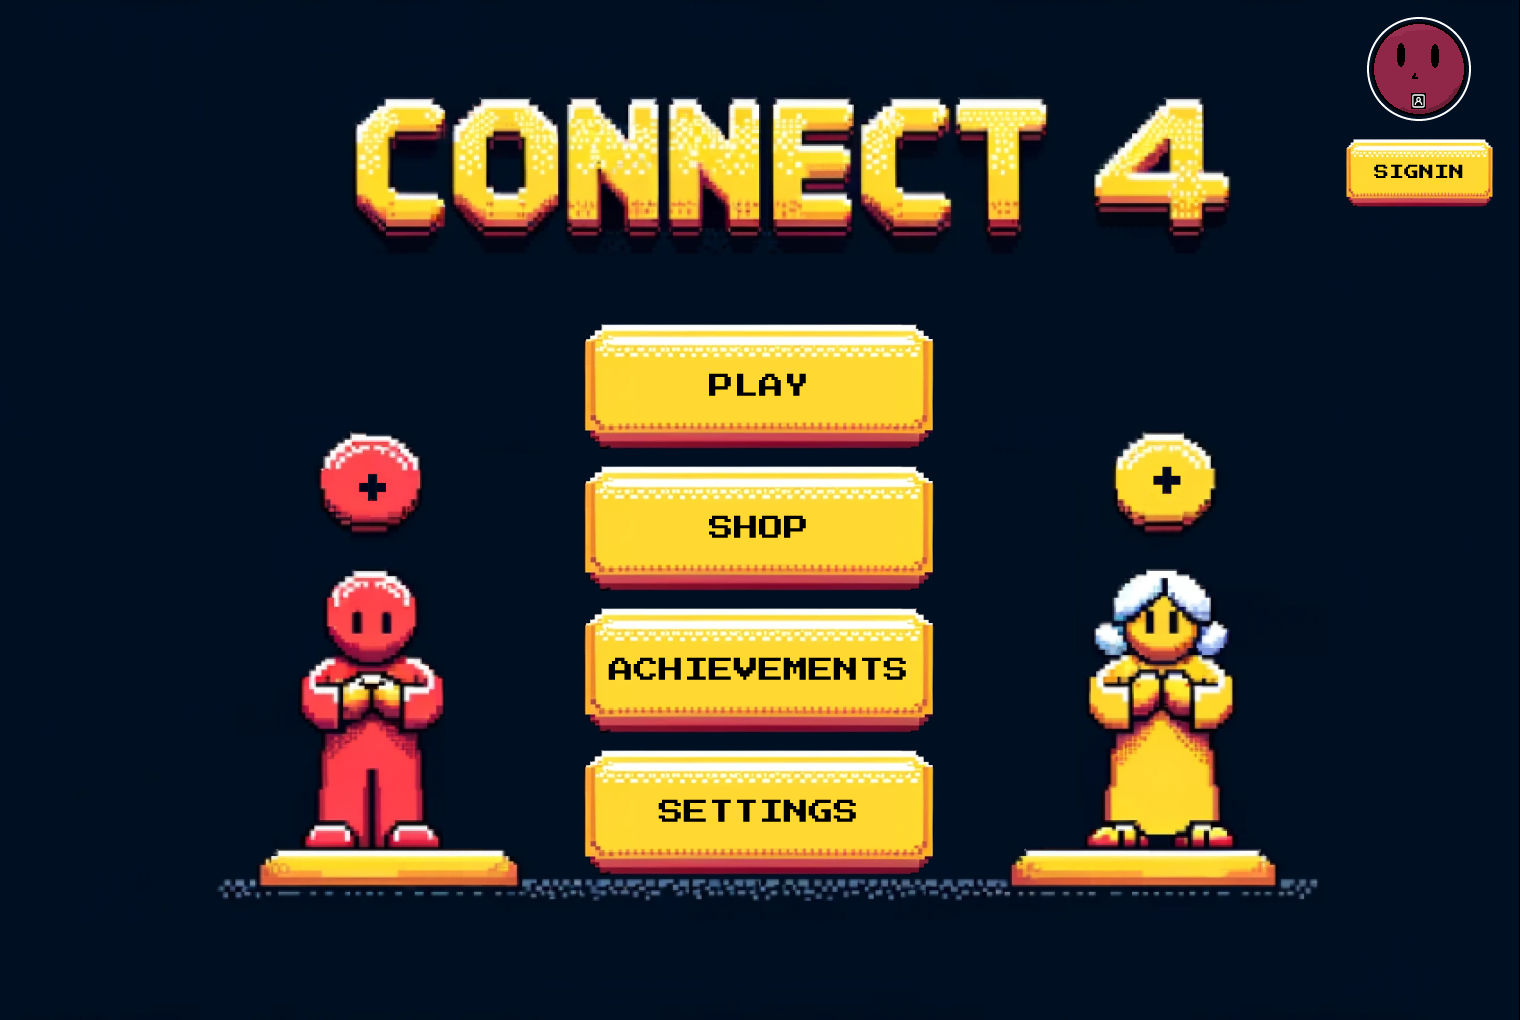
\includegraphics[width=0.8\textwidth]{Menu.png}
  \caption{ Menu hry.}
  \label{fig:menu_label}
\end{figure}

\subsection{Hracia plocha:}
\begin{figure}[H]
  \centering
  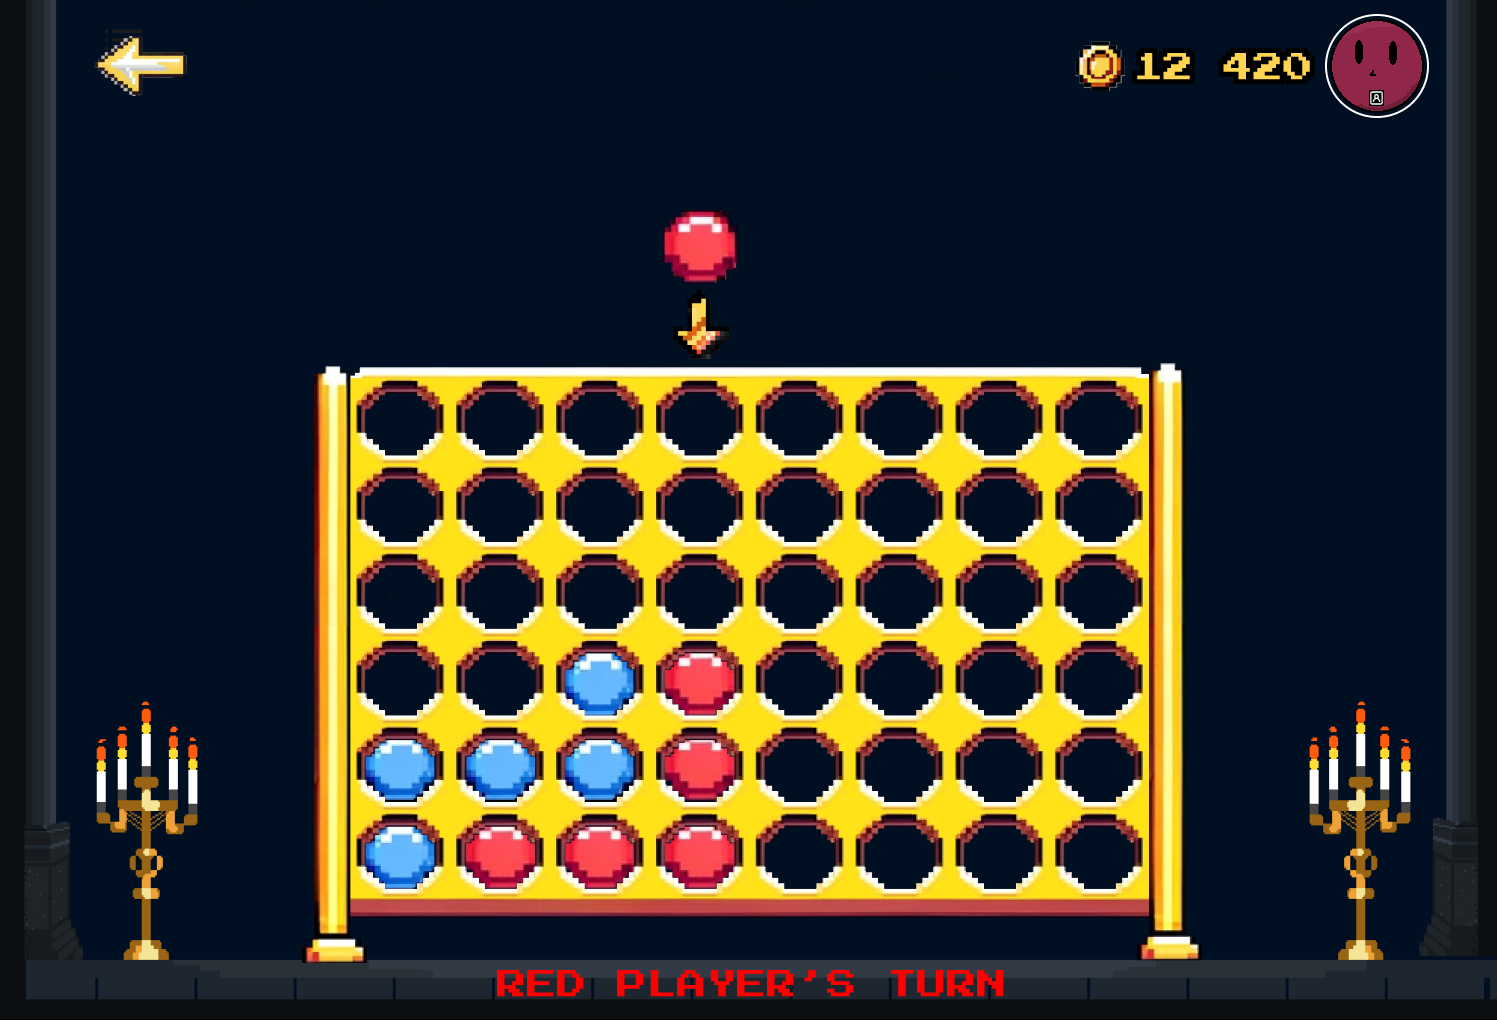
\includegraphics[width=0.8\textwidth]{Plocha.png}
  \caption{ Hracia plocha pre štandardnú verziu.}
  \label{fig:štandard_label}
\end{figure}

\subsection{Modálne okno sumarizácie hry:}
\begin{figure}[H]
  \centering
  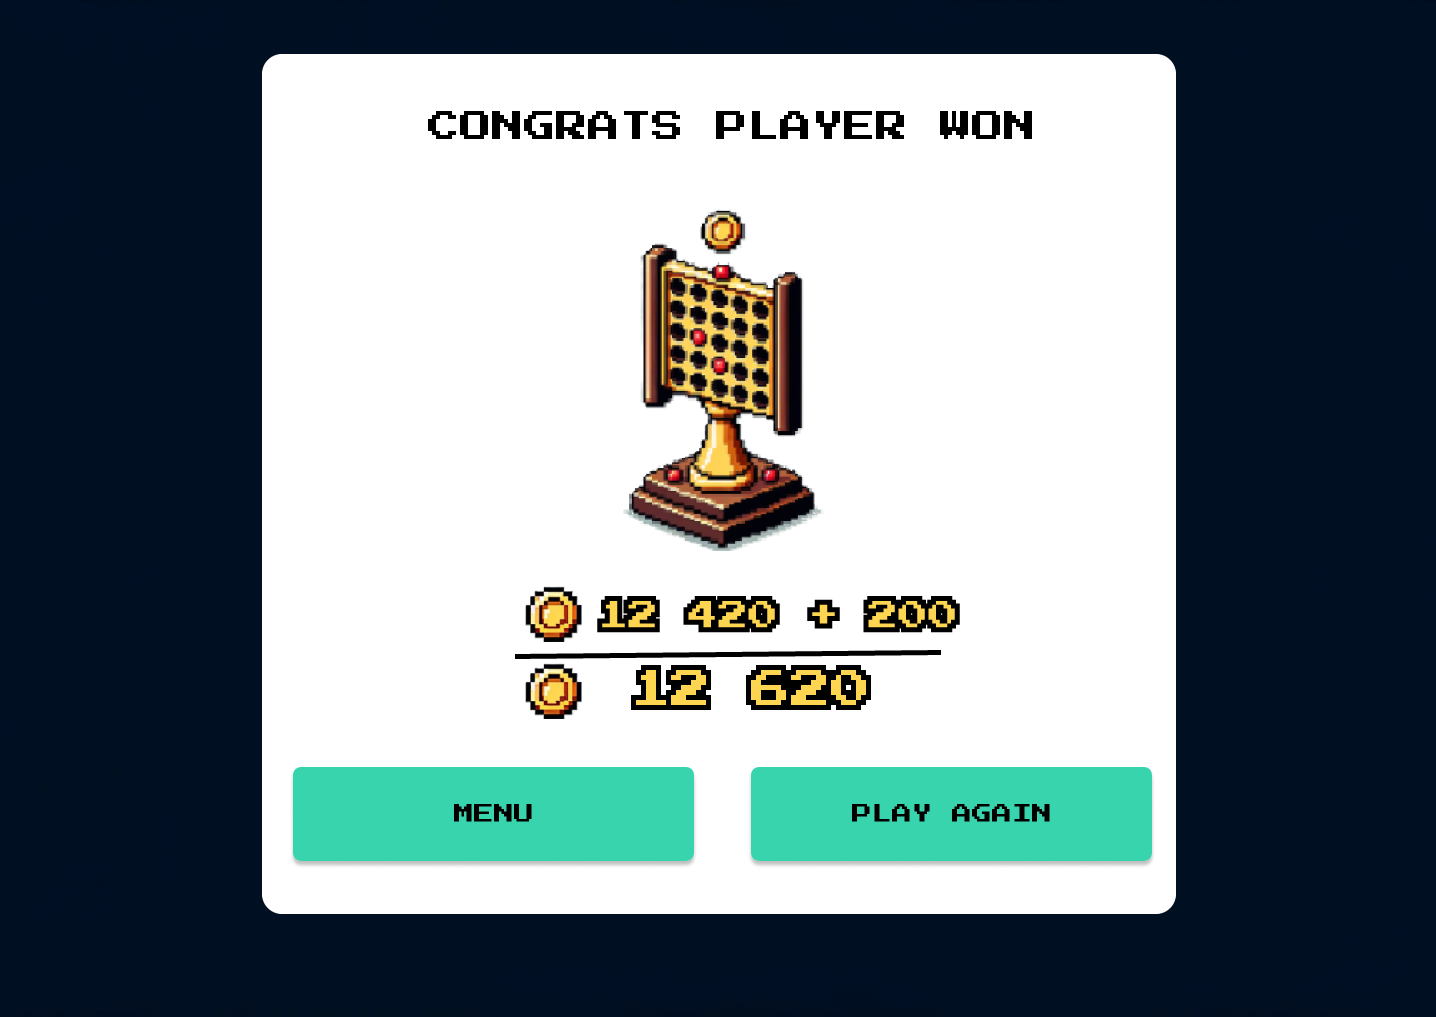
\includegraphics[width=0.8\textwidth]{Vyhra.png}
  \caption{ Sumár po odohraní partie.}
  \label{fig:sumár_label}
\end{figure}

\subsection{Riešenie potrieb užívateľov}
Jakub Majer:
Ivan Mahút:
Dušan Slúka:
\begin{enumerate}
    \item \textbf{Zlepšenie užívateľského rozhrania:} Makety znázorňujú, že sme aktualizovali užívateľské rozhranie hry "Connect 4" s cieľom zvýšiť jeho intuitívnosť a vizuálnu atraktivitu. Rozloženie menu a možnosti sú jasne definované a prístupné.
    \item \textbf{Zlepšenie grafiky a vizuálnych efektov:} Namiesto nudných a už zaužívaných prvkou sme sa rozhodli pre viacej atraktívnejšiu formu uživaťeľského prostredia ktorou je "pixelart". Táto voľba nám dovolila si vo vlastnej réžií navrhnúť a nakresliť väčšinu prvkov čo vyustilo k estetickému dizajnu.
    \item \textbf{Možnosť hrať s priateľmi:} Hra je navrhnutá tak aby vedeli dvaja hráči hrať na jednom zariadení a intuitívne zistili v akom štádiu hra je a čo robiť.
\end{enumerate}

\subsection{Kľúčové problémy a riešenia}
Jakub Majer:
Ivan Mahút:
Dušan Slúka:
\begin{itemize}
    \item \textbf{Slabé užívateľské rozhranie:} Nové užívateľské rozhranie je jasné a intuitívne, zamerané na zlepšenie skúsenosti hráča.
    \item \textbf{Nedostatok herných režimov:} V aktuálnej verzí sú dostupné dva herné režimy pre ktoré sú vytvorené pre dlhšie udržanie a väčšiu návratnosť hráča.
\end{itemize}


\section{Testovanie makety}
\section{Test navigácie v rozhraní}


\textbf{Cieľ:} Overiť, či používatelia môžu ľahko a intuitívne navigovať v rozhraní a rýchlo nájsť požadované informácie.

\textbf{Testovacia úloha/scenár:} 
\begin{itemize}
  \item Zahrať štandardnú hru a potom navigovať naspäť do menu alebo zahrať daľšiu a potom následovať do menu.
  \item Nájasť cestu k registrácií uživaťeľa a naspäť do menu.
\end{itemize}

\textbf{Metriky:}
\begin{itemize}
    \item \textbf{Úspešnosť dokončenia scenára/úlohy (success/error rate):} Koľko používateľov bolo schopných úspešne dokončiť úlohu?
    \item \textbf{Počet pokusov o nájdenie informácie (number of trials):} Koľkokrát používateľ klikol alebo navštívil rôzne časti rozhrania, kým našiel správnu informáciu?
    \item \textbf{Počet dotazov od používateľa:} Koľkokrát používateľ požiadal o pomoc alebo mal dotaz týkajúci sa postupu?
    \item \textbf{Úspešnosť nájdenia predpokladanej cesty pri navigácii (expected path):} Sledujte, či používateľ nasledoval predpokladanú cestu k dosiahnutiu cieľa.
\end{itemize}

\textbf{Respondenti:}

Počet: 3 

Poznámka: Rovnaký ako pri dotazníku.

\textbf{Vyhodnotenie metrík:}
\begin{itemize}
    \item \textbf{Úspešnosť dokončenia scenára/úlohy (success/error rate):} 66\%
    \item \textbf{Počet pokusov o nájdenie informácie (number of trials):} V priemere 2.
    \item \textbf{Počet dotazov od používateľa:} V priemere 1.
    \item \textbf{Úspešnosť nájdenia predpokladanej cesty pri navigácii (expected path):} 100\%
\end{itemize}

\textbf{Vyhodnotenie:}
Test odhalil nedostatok pri navigácií do rozhrania registrácie nového uživaťeľa. V aktuálnej verzí sa k tejto obrazovke dostáva cez obrazovku MENU-LOGIN-REGISTER.
Uživaťeľovi to nakoniec došlo no trvalo mu to dlhšie než by som očakával (úloha 2.). Ako riešenie plánujem pridať tlačítko pre registráciu priamo do Menu aplikácie.
Ďaľšia maličkosť nastala pri jednom respondentovy kedy po kliknutí na tlačidlo play sa zamyslel ktorý herný režim vybrať.
A spýtal sa čo znamená crazy house. Pre opravenie tohoto problému plánujem pridať vysvetlivky ktoré sa  zobrazia po nájdení myššou na konkrétnu hernú možnosť.
Kedže som použil tých istých respondentov ako v dotazníku mohol som sa spýtať či si aplikáciu predstavovali takto ?
Odpovede boli kladné. Najviac si pochvaľovali zaujímavý dizajn a možnosť rýchlej hry bez registrácie.

 
\end{document}
